\documentclass[%
oneside,                 % oneside: electronic viewing, twoside: printing
final,                   % draft: marks overfull hboxes, figures with paths
10pt]{article}

\listfiles               %  print all files needed to compile this document

%\usepackage[a4paper, total={6in, 8in}]{geometry}
\usepackage[totoc]{idxlayout}   % for index in the toc
\usepackage[nottoc]{tocbibind}  % for references/bibliography in the toc

\usepackage{relsize,makeidx,color,setspace,amsmath,amsfonts,amssymb}
\usepackage[table]{xcolor}
\usepackage{bm,ltablex,microtype}
\usepackage{comment} 
\usepackage[pdftex]{graphicx}

\usepackage{fancyvrb} % packages needed for verbatim environments

\usepackage[T1]{fontenc}
%\usepackage[latin1]{inputenc}
\usepackage{ucs}
\usepackage[utf8x]{inputenc}

\usepackage{lmodern}         % Latin Modern fonts derived from Computer Modern


\usepackage{pgfplotstable, booktabs}

\pgfplotstableset{
    every head row/.style={before row=\toprule,after row=\midrule},
    every last row/.style={after row=\bottomrule}
}





% Hyperlinks in PDF:
\definecolor{linkcolor}{rgb}{0,0,0.4}
\usepackage{hyperref}
\hypersetup{
    breaklinks=true,
    colorlinks=true,
    linkcolor=linkcolor,
    urlcolor=linkcolor,
    citecolor=black,
    filecolor=black,
    %filecolor=blue,
    pdfmenubar=true,
    pdftoolbar=true,
    bookmarksdepth=3   % Uncomment (and tweak) for PDF bookmarks with more levels than the TOC
    }
%\hyperbaseurl{}   % hyperlinks are relative to this root

\setcounter{tocdepth}{2}  % levels in table of contents

% --- fancyhdr package for fancy headers ---
\usepackage{fancyhdr}
\fancyhf{} % sets both header and footer to nothing
\renewcommand{\headrulewidth}{0pt}
\fancyfoot[LE,RO]{\thepage}
% Ensure copyright on titlepage (article style) and chapter pages (book style)
\fancypagestyle{plain}{
  \fancyhf{}
  \fancyfoot[C]{{\footnotesize \copyright\ 1999-2018, "Computational Physics I FYS3150/FYS4150":"http://www.uio.no/studier/emner/matnat/fys/FYS3150/index-eng.html". Released under CC Attribution-NonCommercial 4.0 license}}
%  \renewcommand{\footrulewidth}{0mm}
  \renewcommand{\headrulewidth}{0mm}
}
% Ensure copyright on titlepages with \thispagestyle{empty}
\fancypagestyle{empty}{
  \fancyhf{}
  \fancyfoot[C]{{ }}
  \renewcommand{\footrulewidth}{0mm}
  \renewcommand{\headrulewidth}{0mm}
}

\pagestyle{fancy}


% prevent orhpans and widows
\clubpenalty = 10000
\widowpenalty = 10000

% --- end of standard preamble for documents ---


% insert custom LaTeX commands...

\raggedbottom
\makeindex
\usepackage[totoc]{idxlayout}   % for index in the toc
\usepackage[nottoc]{tocbibind}  % for references/bibliography in the toc
\usepackage{listings}
\usepackage[normalem]{ulem} 	%for tables
\useunder{\uline}{\ul}{}
\usepackage{hyperref}
\usepackage[section]{placeins} %force figs in section

\usepackage{natbib}

\usepackage[toc,page]{appendix} % appenix


%-------------------- end preamble ----------------------

\begin{document}

% matching end for #ifdef PREAMBLE

\newcommand{\exercisesection}[1]{\subsection*{#1}}


% ------------------- main content ----------------------



% ----------------- title -------------------------

\thispagestyle{empty}

\begin{center}
{\LARGE\bf
\begin{spacing}{1.25}
Classification and Regression, from linear and logistic regression to neural networks
\end{spacing}
}
\end{center}

% ----------------- author(s) -------------------------

\begin{center}
{\bf Johan Nereng}
\end{center}

    \begin{center}
% List of all institutions:
\centerline{{\small Department of Physics, University of Oslo, Norway}}
\end{center}
    
% ----------------- end author(s) -------------------------

% --- begin date ---
\begin{center}
Nov 13, 2019
\end{center}
% --- end date ---

\vspace{5cm}
\begin{abstract}
-------
\end{abstract}
\newpage




\textit{\textbf{----}} \newline


\textit{\textbf{Authors' comment:} -----}
\newpage

\section{Introduction}
\hyperref[Section_Methods]{methods sections}
\hyperref[Section_Results]{Results}
\hyperref[Section_Discussion_of_results]{discussion of results}
\hyperref[Section_Conclusions]{conclusions}

\hyperref[Section_M_Scaling]{Scaling}
\hyperref[Section_M_Logreg]{Logistic Regression}
\hyperref[Section_M_NN]{Neural Networks}
\hyperref[Section_M_Codeimpl]{Code Implementation}
\hyperref[Section_M_eval]{Evaluating The Implementation}

\textit{autoths: left right mult. confusing in looking at notes, example code and nielsens book}
Regression vs classification
crossvalidation
mean-squared error and/or the R2
or the accuracy score (classification problems) 

Assumes prior knowledge of fundamentals of machine learning, such as what a design matrix, predictors and response is.

A network such as this is a universal approximator, which means that it can approximate any suitably smooth with arbitrary accuracy \citep{MLMurphy}[p.564].
\section{Methods} \label{Section_Theory}

\subsection{Qualitative response modeling}
In this project, both qualitative and quantitative response variables are modeled.  In the case of quantitative \citep{2017introstatlearn}[p.130]. [LOGREG INSTEAD OF LINREG  -EXPLAIN WHY 0-1 etc]


\subsection{Logistic Regression for two classes} \label{Section_M_Logreg}
Logistic regression models the probability that a qualitative response falls within a category. In the case of two mutually exclusive categories or classes, such as "True" ($Y=1$) and "False" ($Y=0$), this translates to modeling the relationship between the probability of $Y=1$ given $X$ as $P(Y=1|X;\beta)=p(X;\beta)$, using the \textit{logistic function} \eqref{eq:logfunc} \citep{2017introstatlearn}[p.132], which due to mutual exclusivity, models $Y=0$ as a function of $X$, or $P(Y=0|X)=p(X';\beta)$, as $1-p(X;\beta)$.
\begin{equation}
p(Y=1|X, \bm{\beta})= p(\bm{X};{\beta})=\frac{e^{\bm{\beta}\bm{X}}}{1+e^{\bm{\beta}\bm{X}}}
\label{eq:logfunc}
\end{equation}
where $\bm{\beta}=[\beta_0, \beta_1, ... \beta_p]$, $\bm{X}=[1,X_1, X_2, ... X_p]$, and $p$ is the number of predictors that the the binary response $Y$ is modeled upon. When fitting the model (estimating the $\beta$ coefficients) to a data set $\mathcal{D}=\{y_i,\bm{x}_i\}_{i=1}^n$, of $n$ observations, the desired fit is the one where the predicted probabilities of $p(\bm{x}_i)$  most precisely corresponds to $y_i$. In other words, one seeks the model which has the highest probability of predicting the data set, which is achieved by utilizing the \textit{maximum likelihood} method \eqref{eq:max_likelihood}\citep{2017introstatlearn}[p.133]. 



\begin{equation}
P(\bm{\beta})=\displaystyle\prod_{i:y_i=1}p(\bm{x}_i; \bm{\beta}) \displaystyle\prod_{i':y_{i'}=0}(1-p(\bm{x}_{i'}; \bm{\beta}))
\label{eq:max_likelihood}
\end{equation}

Taking the log of the maximum likelihood, one obtains the log-likelihood. The (reordered) negative log-likelihood constitutes the cost function, $\mathcal{C}(\hat {{\beta}})$ \eqref{eq:cost_log} \citep{HastieTrevor2009TEoS}[p.120] (in Hastie et al, the log-likelihood is maximized) of the logistic regression, or the \textit{cross entropy}. When minimized, this convex function yields the desired $\beta$ estimates.

\begin{equation}
\mathcal{C}(\bm{\beta})=-\sum_{i=1}^n \left(y_i({\bm{\beta}}\bm{x}_i)-log(1+e^{{\bm{\beta}}\bm{x}_i})\right)
\label{eq:cost_log}
\end{equation}

\subsection{Gradient Decent}  \label{Section_M_GD}
The minimization of a cost function may in some cases be carried out analytically, for example when using least squares error. For some cost function however, the analytic expression may be inconvenient to use. Factors such as the size of a matrix which requires inverting may be to computationally intensive, and in yet other cases, close form solutions are entirely unavailable. For problems such as these, numerical methods for obtaining the desired model fit is instead applied. One such method is the gradient descent (GD) \eqref{eq:GD} \citep{MLMurphy}[p.247], also known as steepest descent. When utilizing GD, one makes an initial guess for $\bm{\beta}$, evaluates the gradient, $\bm g$ of the cost function in order to obtain an estimate closer to the desired minimizing value. This process is then iteratively repeated till the sufficient convergence of the coefficients is reached. In order to not overshoot the $k+1$'th estimate, a \textit{learning rate} of $\eta$ is applied to the gradient - which may also serve to lengthen the step in an iteration. The value of the learning rate can either be fixed, usually by trial and error, such that it works well for the problem at hand, or it may be adapted to each step. 

\begin{equation}
\bm{\beta}_{k+1}=\bm{\beta}_{k}-\eta_k  \bm g (\bm{\beta}_k)
\label{eq:GD}
\end{equation}

For logistic regression, $\bm g$, may be expressed as: \citep{MLMurphy}[p.247]:
\begin{equation}
\bm g (\bm \beta)= \frac{\partial \mathcal{C}(\bm{\beta})}{\partial \bm \beta}= -\hat{X}^T(\bm y-\bm p )
\end{equation}
Where $\hat{X}$, is the design matrix, and $\bm p$ a vector with elements $p(y_i|x_i;\bm \beta)$. \newline

A common improvement on GD is the stochastic gradient descent (SGD), which involves splitting the data into min batches, then randomly selecting one batch at a time from which to compute the gradient. More detailed information is available in literature such as Kevin P. Murphy's book on machine learning \citep{MLMurphy}[p.262].

\subsection{Neural Networks} \label{Section_M_NN}
\textit{For simplicity's sake, matrices are denoted without bold font or hats from here on forwards.} The feed forward neural network (FFNN), or multi-layer perceptron model (MLP), is an artificial neuron network consisting of an ordered series of regression models with connected inputs and outputs \citep{MLMurphy}[p.563]. The network consists of $L$ layers, with  a number of neurons (regression models), or nodes, in each layer. The neurons are not necessarily of the same type, as one can for example use logistic regression models for all nodes but the ones in $L$, which could be linear regression models if the problem is a regression problem. The outputs, $a^1$, of the $M_1$ nodes in layer $l=1$ (one), the input layer, are fed to the nodes in layer $l=2$, and so on, until the outputs, $a^{L-1}$, from layer $l=L-1$ is fed to layer $l=L$, the output layer. Outputs from layer $L$, $a^L$ are the network's outputs, and predict the target(s) of the model. The layers in-between layer $1$ and layer $L$, are deterministic functions of the input, and are called hidden layers.  Each node in each layer uses weights for each input, similar to the coefficients  corresponding to the predictors described in the \hyperref[Section_M_Logreg]{logistic regression subsection}. In addition, each node has it's own \textit{bias}, $b$, which regulates the output tendency of neuron. The sum of the weighted inputs and the bias, $z$, is usually called the activation of the neuron, not to be confused with it's output. The output is however a function of the activation, such that $a^l=f^l(z^l)$, where $f(z)$ is called an activation function. \newline

\textit{The remaining subsections on neural networks are based on the informative and well written book by Michael Nielsen book \citep{Nielsen15} (using a slightly different matrix indexation than what this project does), and lectures notes in   FYS-STK4155 \cite{MHJ_NN}}.
\subsubsection{Feed forward}
The propagation of neuron outputs in the network, resulting in prediction, is called feed forward. The network used in this project is set up such that it takes  $n_{inputs}$ observations, of $n_{predictors}$ predictors, thus working through the entirety of the data in one go. As with other regression methods, the design matrix $X$ ($n_{inputs} \times n_{predictors}$) is the input, which in the end outputs a matrix $ y$ ($n_{inputs} \times n_{targets}$) of predicted values for the $n_{targets}$ targets. By arranging the weights of layer $l$, $w^l$ ($M_{l-1} \times M_l$), the activations of layer $l$ is calculated by $z_l=X w^l$ ($n_{inputs} \times M_l$). Taking $a^l=f^l(z^l)$ ($n_{inputs} \times M_l$), means that $a^l$ holds the output for every neuron in $l$. 

\subsubsection{Cost function and backpropagation} \label{Section_M_NN}
Once $a^L$ is obtained through the feed forward process, the network has made a prediction on the target(s), $y$, for each of the $n_{inputs}$ observations. However, unless one has divine insights, initiating the weights and biases such that $a^L \approx y$ with sufficient accuracy is unlikely. The quality of these  predictions is quantified by the cost function $C(w,b)$, which as indicated is a function of the weights and biases of network. The effect on prediction quality when adjusting $w$ and $b$ is thus measurable by the cost function, which, as in the case of the logistic regression, is to be minimized. In the case of FFNNs, this is done through backpropagation, which is the process of calculating the error of each layer, \eqref{eq:BP1} and \eqref{eq:BP2}, and the gradient of the cost, $\nabla C$, function w.r.t the biases \eqref{eq:BP3} and weights \eqref{eq:BP4}. 
\begin{align}
\label{eq:BP1} &\delta_L=\nabla_a C \odot  f' (z^L) \\  
\label{eq:BP2} &\delta_l=\delta^{l+1}(w^{l+1})^T \odot  f' (z^l)\\ 
 \label{eq:BP3} &\frac{\partial C}{\partial b^l} =\delta^l\\ 
\label{eq:BP4} &\frac{\partial C}{\partial w^l} =(a^{l-1})^T \delta^l 
\end{align}

Having obtained the gradient $\nabla C$, \hyperref[Section_M_GD]{gradient decent} is applied in order to calculate new weights and biases. Once the weights and biases are updated, a new feed forward process is initiated, followed by backpropagation and corresponding adjustments of parameters until the cost function is sufficiently minimized or the number of iterations (feed forward + backpropagation) is reached.

\subsubsection{Neural network for classification}  \label{Section_M_NNclass}
In the logistic regression case, this project did not use one hot encoding - using  cross entropy ensures equal importance of both target options when training. For the NN implementation however, one-hot encoding is used, along with cross entropy \eqref{eq:cost_log} as the cost function. As the one-hot encoding means that the network is expected to output two values, representing the likelihood of each of the two categories for each data point, the activation function of the output layer is the softmax function \eqref{eq:softmax} (output of neuron $j=1,2$ in $L$), which normalizes the sum of the outputs to one. 

\begin{equation}
a_j^L= \frac{e^{z_j^L}}{\sum e^{z^L}}
\label{eq:softmax}
\end{equation}
Using the cross entropy as the cost function, sigmoid for hidden layer(s), and softmax as the activation for layer $L$, means that the backpropagation equations \eqref{eq:BP1}-\eqref{eq:BP4} for the two last layers of network are:
\begin{align*}
&\delta_L=a_L-y \\   
&\delta_{L-1}=\delta_L(w^{L})^T \odot  a_{L-1} \odot (1- a_{L-1})\\ 
&\frac{\partial C}{\partial b^L} =\delta^L\\ 
&\frac{\partial C}{\partial w^L} =(a^{L-1})^T \delta^{L}  \\
&\frac{\partial C}{\partial b^{L-1}} =\delta^{L-1}\\ 
&\frac{\partial C}{\partial w^{L-1}} =(a^{L-2})^T \delta^{L-1} 
\end{align*}
It's worth noting that in the output error, when using softmax with cross-entropy, the $f'(z)$ term cancels with parts of the derivative of $C$ w.r.t $a$.
\subsubsection{Neural network for regression}
In this project, the neural network for regression is set up using the quadratic cost, with $tanh (z)$ as activation function in hidden layer(s), and with $f(z^L)=z^L$, the identity activation, as activation for the output layer. Due to the change in activation functions, the backpropagation changes slightly, however, as the cost function is also changed, the output error remains the same.

\begin{align*}
&\delta_{L-1}=\delta_L(w^{L})^T    \odot (1-tanh(z_{l-1}^2)) \\ 
\end{align*}

\subsection{Implementation, testing, and evaluation}
Logistic regression for classification is implemented in it's own program using python 3.7.5. The program also uses functionalities from scikit-learn \cite{sklearn} for splitting data into test and training sets, metrics such as producing a confusion matrix, and scaling functions. A neural network for classification is also implemented, building on the template provided in the lecture slides on neural networks from the course FYS-STK4155 \cite{MHJ_NN}. The neural network uses one hidden layer, and activation functions and cost functions as described in the subsection on \hyperref[Section_M_NNclass]{neural networks for classification}. 

\paragraph{Initial testing} of the logistic regression model is carried out on data from the breast cancer data set available through scikit-learn, which contains 569 data points with 30 predictors and targets ($212$ WDBC-Malignant, $ 357$
WDBC-Benign), using both GD and SGD. The program features an option to plot (set plot=True in function call for GD or SGD) the cost function vs. number of iterations and epochs (time) for GD and SGD respectively - which shows that the cost function decreases with iterations/epochs, thus indicating a working implementation.  Having established implementation integrity, the project now moves on to evaluation.

\paragraph{Evaluation of accuracy}
The accuracy score of a classifier \eqref{eq:accuracy}, where $I$ is the indicator function, reflects the number of correctly predicted targets $t_i$ - where a perfect classifier will have a score of $1$. 
\begin{equation}
\text{Accuracy}=\frac{\sum_{i=1}^{i=n}I(t_i=y_i)}{n}
\label{eq:accuracy}
\end{equation}
area ratio score
\subsection{Preprocessing}
Invalid entries in the categorical predictors are removed from the data all together. Then, the categorical predictors that may take on more other values than $0$ and $1$ are one-hot encoded - the remaining categorical predictors are kept as they are with the intention of limiting the number of predictors. After having done so, the features are standardized by substracting the mean and scaling to unit variance.  Having done so, the dat is split into test and training, using a stratified split, ensuring integrity of target category ratio in training and test sets. Before training the model however, there is the accute issue of skewness - the number of observations on default is too low for their effect on 

with/without smote!


In order to better train the machine learning algorithms, a number of methods a
remove outliers,  one hot encoding categories, stratified split, Scaling, smote (upsampling of y), train, predict
\subsection{Scaling} \label{Section_M_Scaling}
 \label{Section_M_Matrixrep}
In order to write a program using logistic regression with gradient decent, matrix representation greatly greatly improves readability and effectiveness. 



\subsection{Code Implementation} \label{Section_M_Codeimpl}
\subsection{Evaluating The Implementation} \label{Section_M_eval}

\subsubsection{Preprocessing}
Scaling, before and after
Stratification, before and after
\section{Results} \label{Section_Results}
\ref{fig:logreg_no_pp} shows the gains chart produced by the logistic regression program on the credit card data with no other pre-processing of the data than one-hot encoding of categorical predictors with values other than 0/1. As the plot suggests, the model performs the same as a random classifier.  
\begin{figure}[!h]
        \centering 
         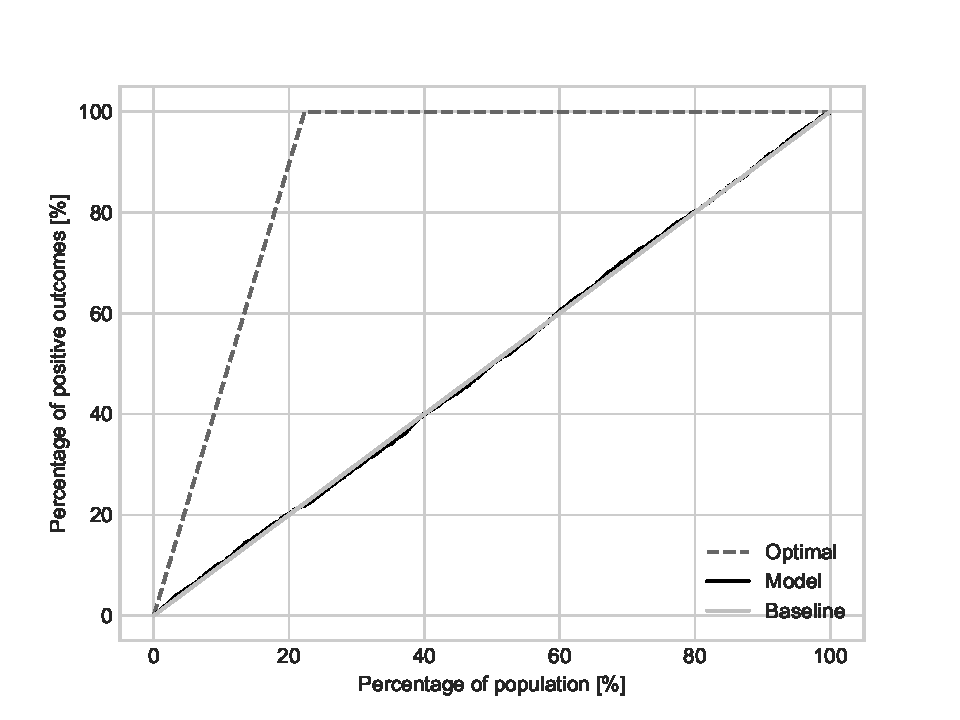
\includegraphics[scale=0.7]{../Results/CC_logreg_no_pp/gains_gd.pdf} 
        \caption{Gains plot for logistic regression using GD with $5000$ iterations and $\eta=0.1$ on credit card data, no pre-processing of data other than one-hot encoding. Accuracy score=$0.78$, Area ratio score=$0.00$}
        \label{fig:logreg_no_pp}   
\end{figure}  

\section{Discussion of results} \label{Section_Discussion_of_results}
\subsection{Implementation, testing, and evaluation}
The accuracy score of the logistic regression model on the raw credit card data (with one-hot encoding) is $0.78$, a deceivingly high score, considering that the area ratio score is $0.00$. This indicates that that the model is classifying all the test data as $0$ ($1$ being defaulting on payment) - which the confusion matrix  \hyperref[Section_M_NNclass]{(see appendix 1.)} confirms. The discrepancy  in evaluation scores shows hat accuracy is not necessarily a meaningful measurement on model performance, especially when the whole goal of the operation is to, in the case of the credit card data, evaluate who will default. It is not unreasonable to imagine that one would prefer a model which produces a few false default flags over on which produces too few.
\section{Conclusions} \label{Section_Conclusions}


\bibliography{ref}
\bibliographystyle{plain}


\begin{appendices}
\section*{Appendix 1.} \label{APP_1}
\end{appendices}
Confusion matrix for linear regression classifier on un-processed credit card data.
\begin{equation}
\bm{X}=\begin{bmatrix}
tn=7591 & fp=0 \\
fn=2178  &tp= 0 \\
\end{bmatrix}
\end{equation}
\end{document}